\documentclass[12pt]{beamer}
\usetheme{Pittsburgh}
\usepackage[spanish]{babel}
\usepackage{times}
\usepackage[T1]{fontenc}
\usepackage[utf8]{inputenc}
\usepackage{graphicx}
\usepackage{tikz}
\usepackage{listings}

\usepackage{pgfpages}
\pgfpagesuselayout{2 on 1}[a4paper,border shrink=5mm]

\renewcommand\shorthandsspanish{}
\noextrasspanish

\title{Curso de Matlab.  Nivel Básico}
\author{Guillem Borrell i Nogueras}

\begin{document}

\lstset{language=Matlab,
  backgroundcolor=\color{black!10},
  numbers=left,
  basicstyle=\small\ttfamily,
  keywordstyle=\color{blue},
  extendedchars=true,
  inputencoding=utf8,
  showspaces=false}

\begin{frame}
  \titlepage
\end{frame}

\begin{frame}
  \frametitle{Yo.}
  \begin{itemize}
  \item Guillem Borrell i Nogueras.
  \item Ingeniero Aeronáutico (aunque no me gustan los aviones).
  \item Becario del Grupo de Investigación de Mecánica de Fluidos
    Computacional de la Universidad Politécnica de Madrid.
  \item Consultor Senior de Englobe Technologies.
  \item \textit{I Have Become Comfortably Numb},
    \url{http://torroja.dmt.upm.es/guillem/blog/}
  \item \textit{Introducción Informal a Matlab y Octave},
    \url{http://iimyo.forja.rediris.es/}
  \end{itemize}
\end{frame}

\begin{large}

\begin{frame}
  \frametitle{¿Qué es Matlab?}
  \begin{itemize}
    \item{Un lenguaje de programación}
    \item{Un lenguaje de programación \emph{interpretado}}
    \item{Un lenguaje de programación \emph{interactivo}}
  \end{itemize}
  \begin{center}
    \textbf{Usar Matlab == Programar en Matlab}
  \end{center}
\end{frame}

\begin{frame}
  \frametitle{¿Qué no es Matlab}
  \begin{itemize}
    \item Una hoja de cálculo
    \item Un programa de cálculo simbólico.  Matlab puede hacer
      $\int_0^1 erf(x)\ dx = 0.486$ pero no 
      $\int erf(x)\ dx = x\ erf(x)+\frac{e^{-x^2}}{\sqrt{\pi}}$
    \item La solución a todos nuestros problemas.
  \end{itemize}
\end{frame}


\defverbatim[colored]\testcode{
  \begin{lstlisting}
    >>
  \end{lstlisting}
}

\begin{frame}
  \frametitle{¿Qué significa interpretado?}
  \begin{itemize}
    \item Un intérprete es un programa.
    \item Es como un actor que hace todo lo que le dice un
      \emph{guión}
    \item Muy parecido a la una calculadora.
    \item Es interactivo.
  \end{itemize}
  \testcode
  Os presento a la consola de Matlab
\end{frame}

\begin{frame}
\frametitle{Algunas mentiras}
\begin{itemize}
  \item Para ser ingeniero aeronáutico no es necesario saber
    programar.
  \item Programar es difícil.
  \item Programar \emph{bien} es fácil.
  \item Los ingenieros programan bien
  \item En la vida basta un lenguaje de programación mientras se
    domine.
\end{itemize}
\end{frame}

\begin{frame}
  \frametitle{Un autoengaño}
  \begin{LARGE}
  \begin{center}
    Si en la escuela sólo me dan seis créditos de informática es
    porque no es importante.
  \end{center}
  \end{LARGE}
\end{frame}

\begin{frame}
  \begin{LARGE}
  \begin{center}
    En Arquitectura nadie enseña Autocad.
  \end{center}
  \end{LARGE}
\end{frame}

\begin{frame}
\frametitle{Problema:}
Representar la integral de la función de Bessel

\[ \int_0^y J_{2.5}\ dx \]

con $y \in [1,5]$

\begin{itemize}
\item ¿Cómo se haría en Fortran?
\item ¿Cómo se haría en Excel?
\end{itemize}
\end{frame}

\defverbatim[colored]\testcode{
\begin{lstlisting}
x=linspace(1,5,100);
intbessel=@(y) quad(@(x) besselj(2.5,x),0,y);
for i=1:100
  z(i)=intbessel(x(i));
end
plot(x,z);
\end{lstlisting}
}

\begin{frame}
\frametitle{En Matlab son 6 líneas}
\testcode
No os preocupéis si no entendéis nada.  Esto es Matlab avanzado.
\end{frame}

\begin{frame}
\frametitle{El resultado}
  \begin{figure}[h]
    \centering{}
    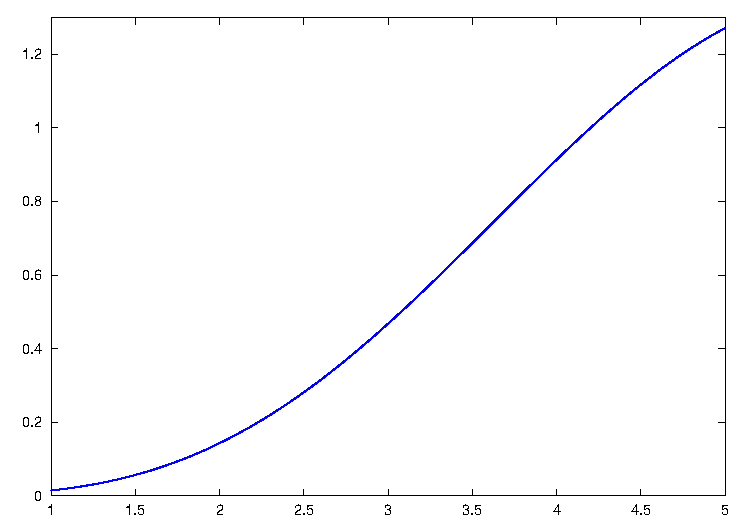
\includegraphics[width=8cm, keepaspectratio]{fig/primera.pdf}
  \end{figure}
\end{frame}


\defverbatim[colored]\testcode{
\begin{lstlisting}
>> 2+2
ans =  4
>> mean([1,2,3,4,5,6,7,8,9])
ans =  5
>> abs(3+4i)
ans =  5
\end{lstlisting}
}

\begin{frame}
  \frametitle{¿Una calculadora programable?}
  \testcode
\end{frame}

\begin{frame}
  \frametitle{Todo esto es muy bonito pero...}
  \begin{itemize}
    \item ¿Es una herramienta realmente útil?
    \item ¿Se usa masivamente en la industria?
    \item ¿Por qué?
    \item ¿Cuánto cuesta Matlab?
    \item ¿Es la única solución?
  \end{itemize}
\end{frame}

\begin{frame}
  \frametitle{Octave}
  \begin{itemize}
    \item Implementación libre y gratuita del lenguaje Matlab
    \item \url{http://www.octave.org}
    \item Programa muy utilizado en GNU/Linux
    \item Versiones para Windows y Mac
    \item QtOctave
    \item \emph{Libre y gratuito}
  \end{itemize}
\end{frame}

\begin{frame}
  \frametitle{El lenguaje Matlab}
  \begin{itemize}
    \item Caracteres especiales
    \item Funciones y scripts
    \item Tipos
    \item Variables
    \item Operadores
    \item Sentencias
    \item \emph{Function handles}
  \end{itemize}
\end{frame}

\defverbatim[colored]\testcode{
\begin{lstlisting}
>> \% Este comando será ignorado
>> 'hola' \% 'Hola,Matlab!'
ans = hola

>> 'hola';
>> 'hola', 'que tal'
ans = hola
ans = que tal

>> 'hola', ...
'que tal'
ans = hola
ans = que tal
\end{lstlisting}
}

\begin{frame}
\frametitle{Caracteres especiales}
\testcode
\end{frame}

\end{large}

\end{document}
